\documentclass{article}
\usepackage{amsmath}
\usepackage{graphicx}
\usepackage{listings}
\newcommand{\includecode}[2][c]{\lstinputlisting[caption=#2, escapechar=, language=#1]{#2}}

\begin{document}
\lstset{language=C} 
\title{Update: Introducing Dynamic Walls in an Integer Lattice Gas Simulation}
\author{David Jedynak}
\maketitle
\begin{abstract}
<<<<<<< HEAD
The purpose of this project is to integrate dynamic shapes into an Integer Lattice Gas Simulation. Currently, vertical lines have been created which can move and simulate particles being pushed. The momentum imparted on the wall has been calculated and the wall velocity dependent on particle collisions have been achieved. The next features being worked on are the additions of multiple lines(vertical, horizontal, and diagonal). This feature should make it easy to create different dynamic shapes out of several lines.   
=======
The purpose of this project is to integrate dynamic shapes into an Integer Lattice Gas Simulation. Currently, vertical lines have been created which can move and simulate particles being pushed. The momentum imparted on the wall has been calculated and the wall velocity dependent on particle collisions has been acheived. The next features being worked on parameterizing the additions of multiple lines(vertical, horizontal, and diagonal). This feature should make it easy to create different dynamic shapes out of several lines. 
>>>>>>> 1e1b30a4df3ad27c758e98ed13c6c904fd4f09cb
\end{abstract}
\section{Problem Description}
The lattice gas code simulation is currently unable to model systems with dynamic solid objects. Having the feature to add movable walls would allow for simulation of interactions between solid physical objects and gasses. The project will begin with simple moving walls that will influence particle dynamics, but the particles will not influence the walls dynamics. Afterwards, implementing wall momentum dependent on particle collisions will be developed. There are some questions on to compensate for limited particle velocities(-1,0,+1) in the LG2d simulation. When a wall and a particle collide and they have opposite velocities, how does the particle reflect and keep momentum conserved? The particle currently can't have a velocity magnitude greater than 1. Perhaps the LGd2 simulation would require the feature to allow for higher particle velocities.
\section{Methods}
<<<<<<< HEAD
The primary objective is to have a shape/line/wall that can move and appear to push lattice gas particles like a physical wall would do in the real world. These walls in the existing program can be easily moved, but as the wall moves it will move through some particles creating a leakage. To compensate for this leakage, particles are subtracted from the lattice sites on the leaving side of the wall and the same number are added to the arriving side of the wall. The sum of the particles added or removed must be zero and it must not create negative particle densities when particles are removed from one side of the wall. The number of particles added is taken randomly from a flat distribution. 
\section{Research Group}
David Jedynak is the only undergrad working on this project.
\section{Completed Milestones}
\begin{itemize}
  \item Simulate with stationary wall and particles initially moving uniformly perpendicular to the wall. Observe how the wall influences the particles' average velocity.
 
    
  \item Develop code to simulate a moving wall(independent of particle collisions). Simulate with initially stationary particles. Observe how the wall influences particles average velocity. Compare results to item 1 on this list. They should have a similar result because both particles and wall are both moving with the same velocity relative to each other.
\begin{figure}

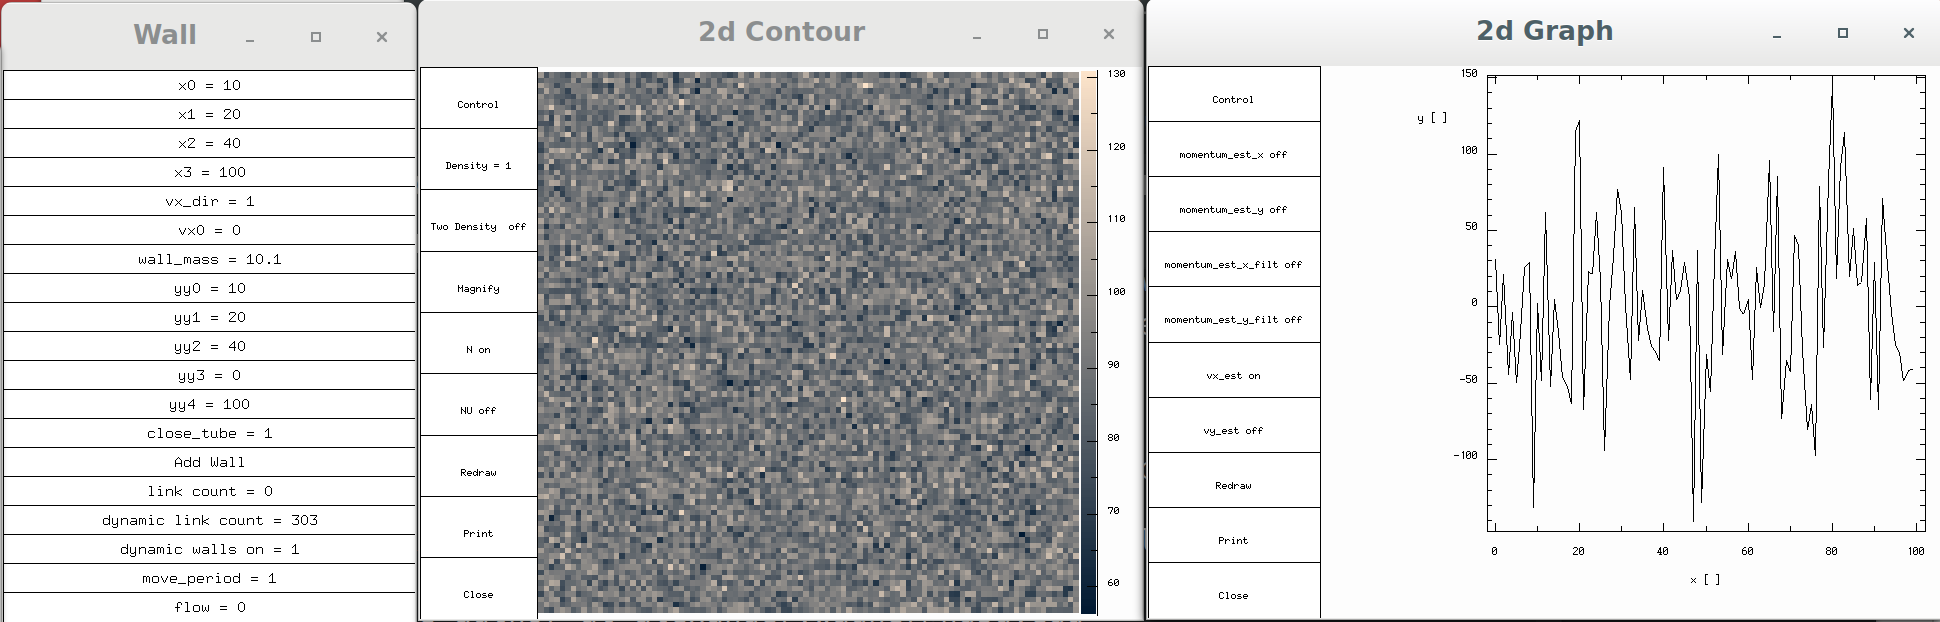
\includegraphics[scale=0.2]{ms1p0.png}
\caption{\label{fig} The 2d graph on the right hand side is the horizontal particle velocity. The contour plot is the Integer Lattice Gas Simulation with an independent moving wall. This is the simulation with the wall velocity being zero.}
\end{figure} 

\begin{figure}

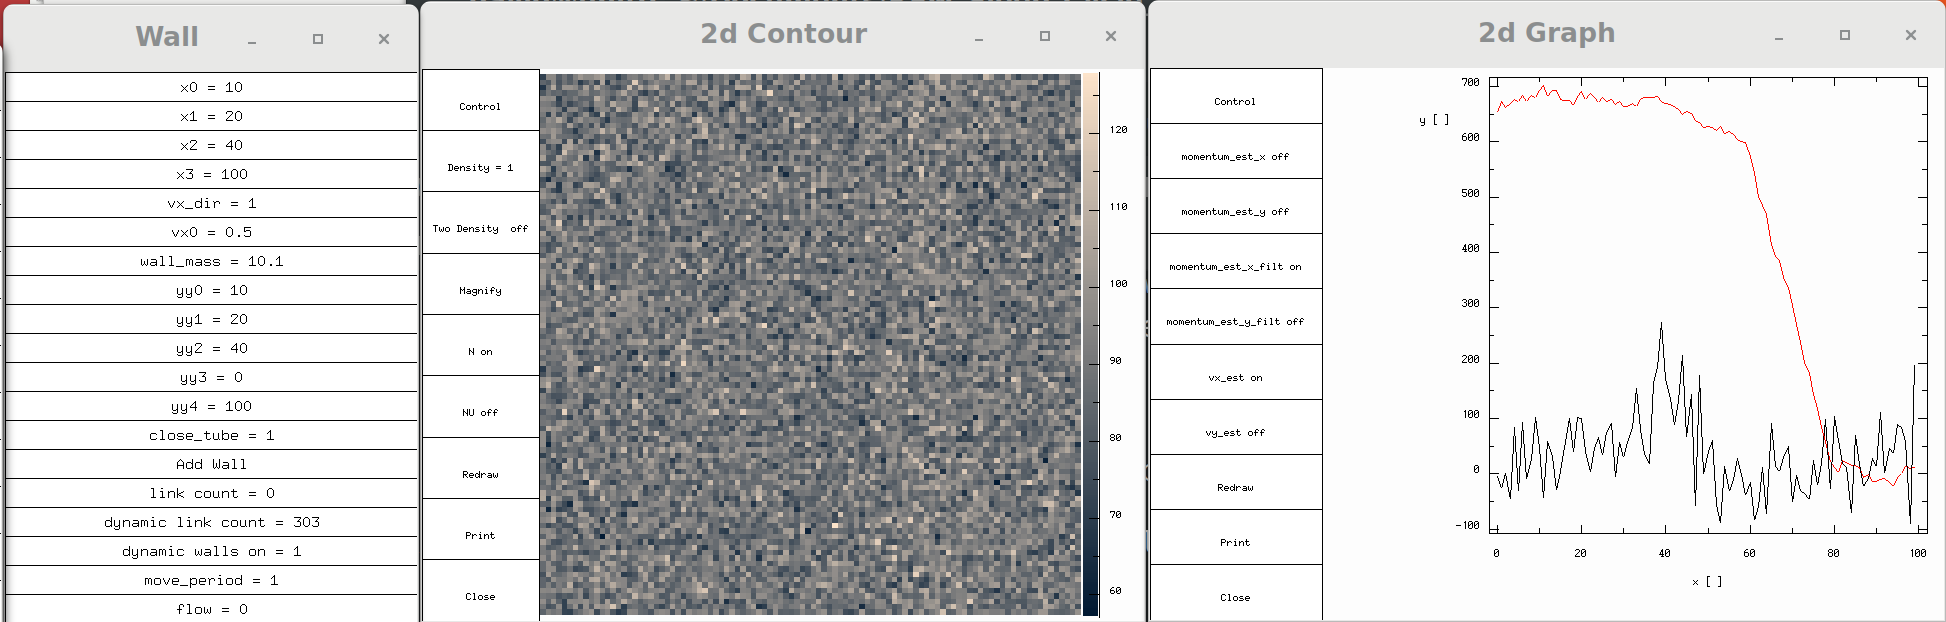
\includegraphics[scale=0.2]{ms1p1.png}
\caption{\label{fig} Several iterations later: the 2d graph on the right hand side is the horizontal particle velocity. The contour plot is the Integer Lattice Gas Simulation with an independent moving wall. This is the simulation with the wall velocity being nonzero(0.5) and positive. Observe how the particle velocity(Black) and Wall momentum (Red) increases.}
\end{figure}

\begin{figure}

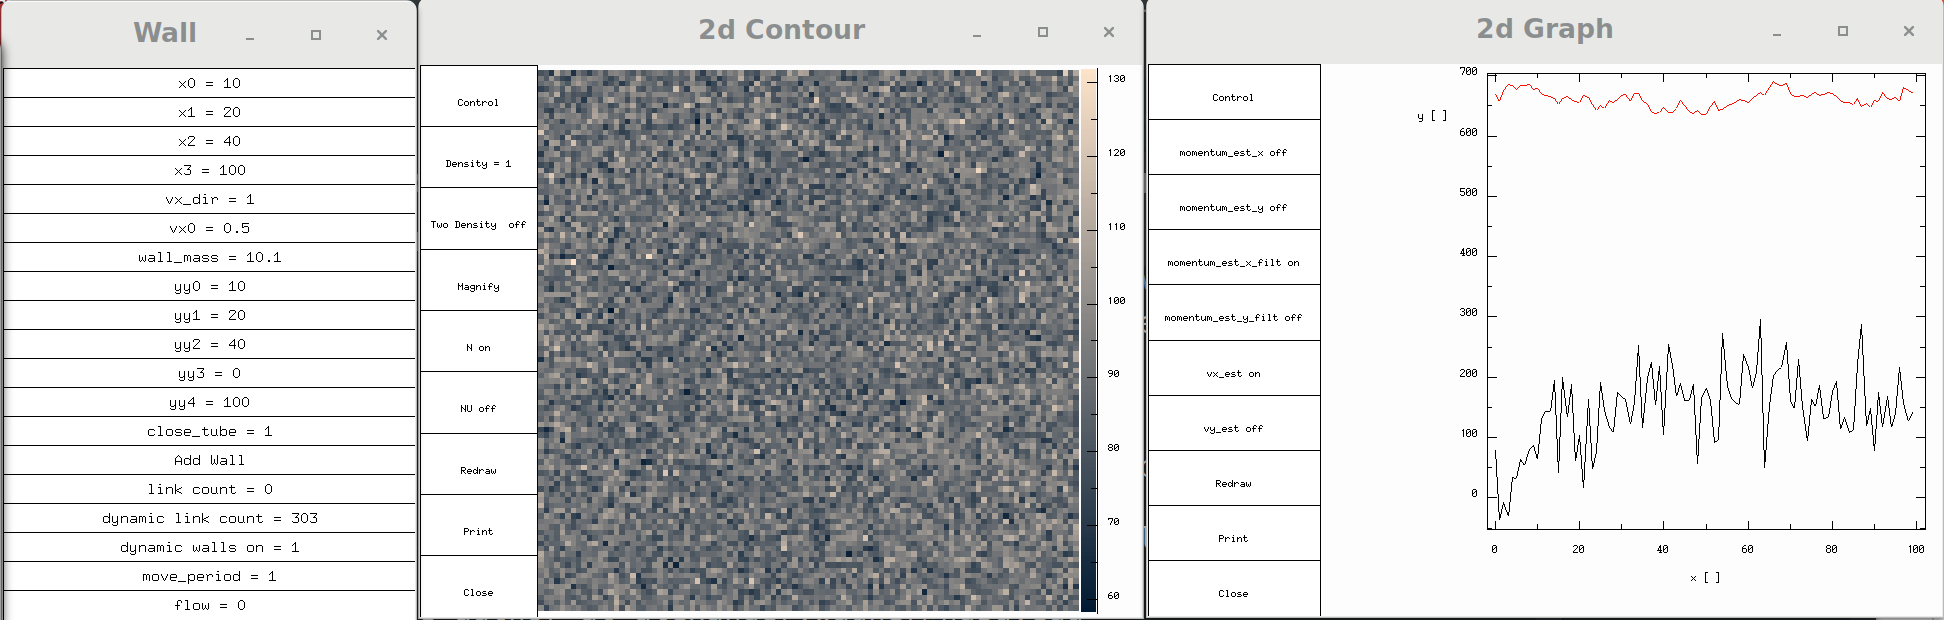
\includegraphics[scale=0.2]{ms1p2.png}
\caption{\label{fig} After running for sometime: The 2d graph on the right hand side is the horizontal particle velocity. The contour plot is the Integer Lattice Gas Simulation with an independent moving wall. This is the simulation with the wall velocity being nonzero(0.5) and positive. The total wall momentum levels off and the particle velocity levels off as well.}
\end{figure}    
 \item Develop code to make wall momentum to be dependent on particle collisions. Simulate a hollow, horizontal, stationary tube with one horizontally movable, vertical wall. place gasses in each side of the vertical wall with different densities. Observe the movement of the movable wall. The wall should stop moving when both particle densities equalize.\newline
\vspace{5mm}\newline
\begin{figure}

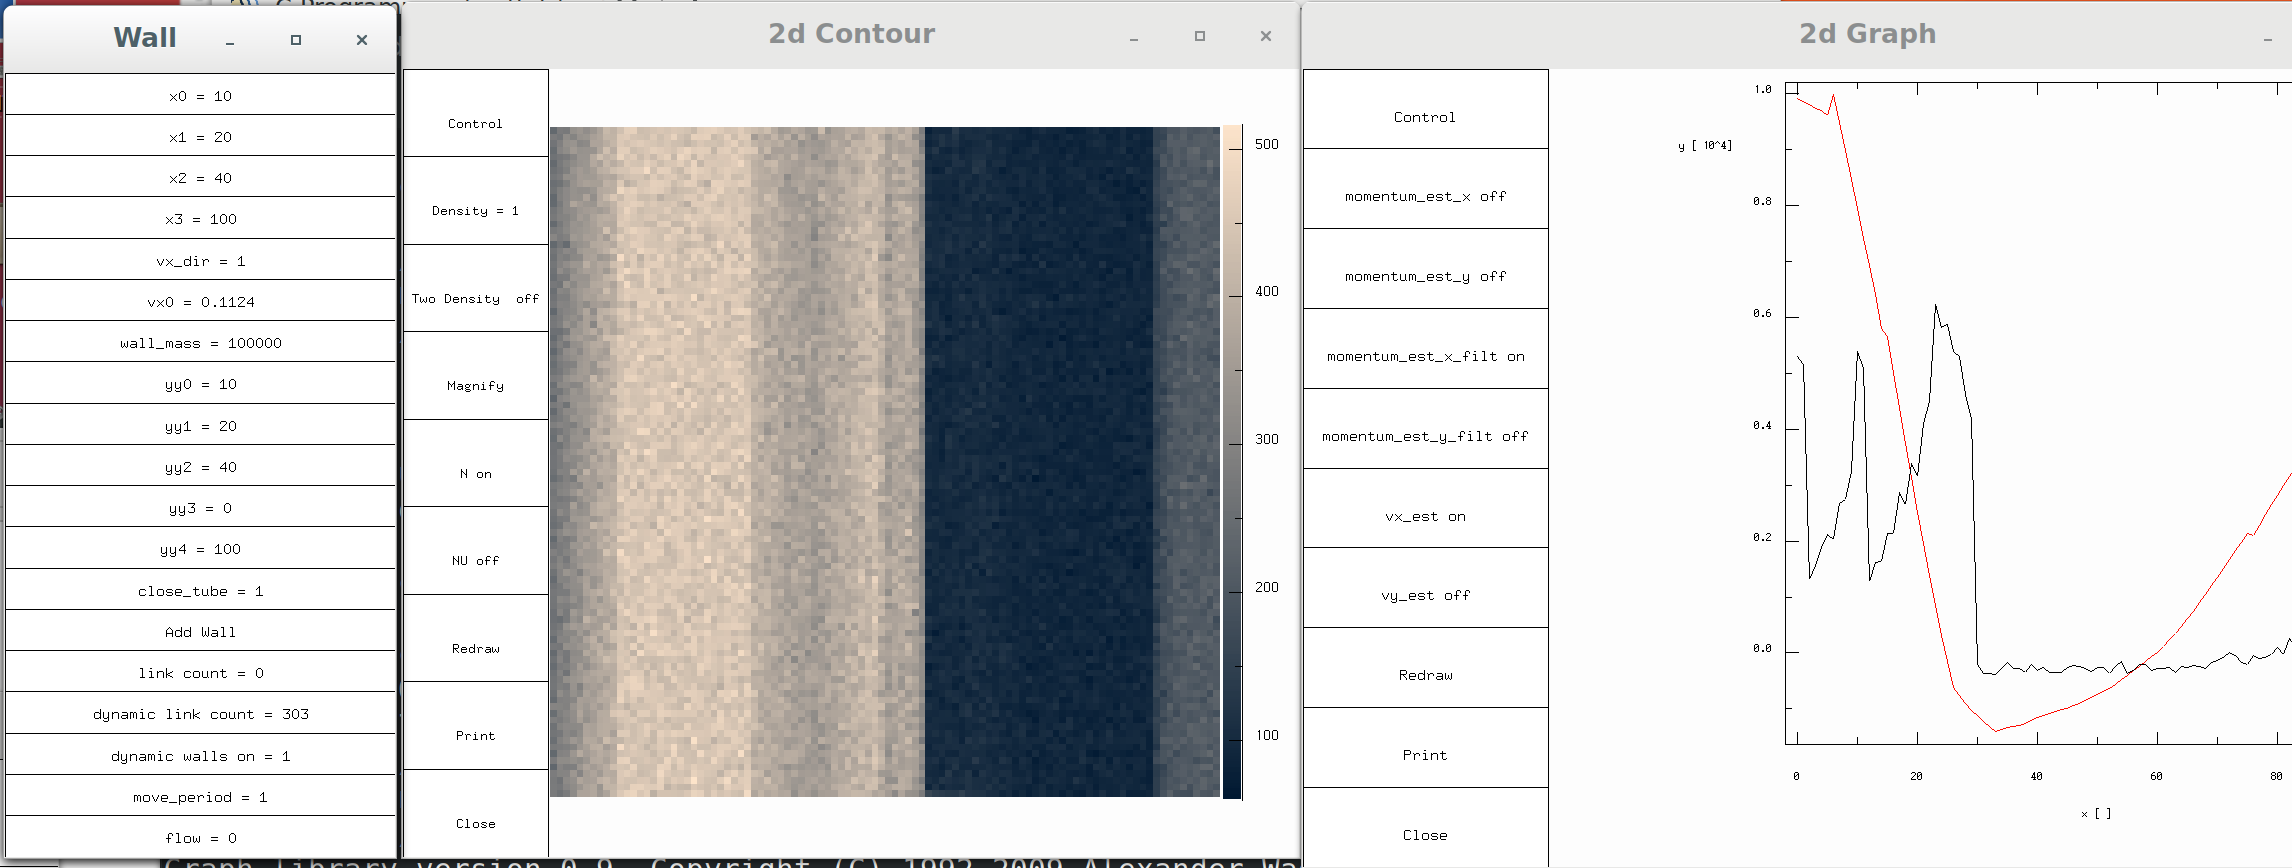
\includegraphics[scale=0.2]{ms2p0.png}
\caption{\label{fig} This is a simulation where the dynamic wall's horizontal velocity is proportional to the momentum gained by the gas particles divided by a set mass. The left hand side has particle densities of 100 from x = 0 to 40 and then densities of 20 from 60 to 100. The purpose of this experiment was to watch the wall velocity change based on particle collisions. See how the velocity (vx0 is equal to ~0.1)}
\end{figure}

\begin{figure}

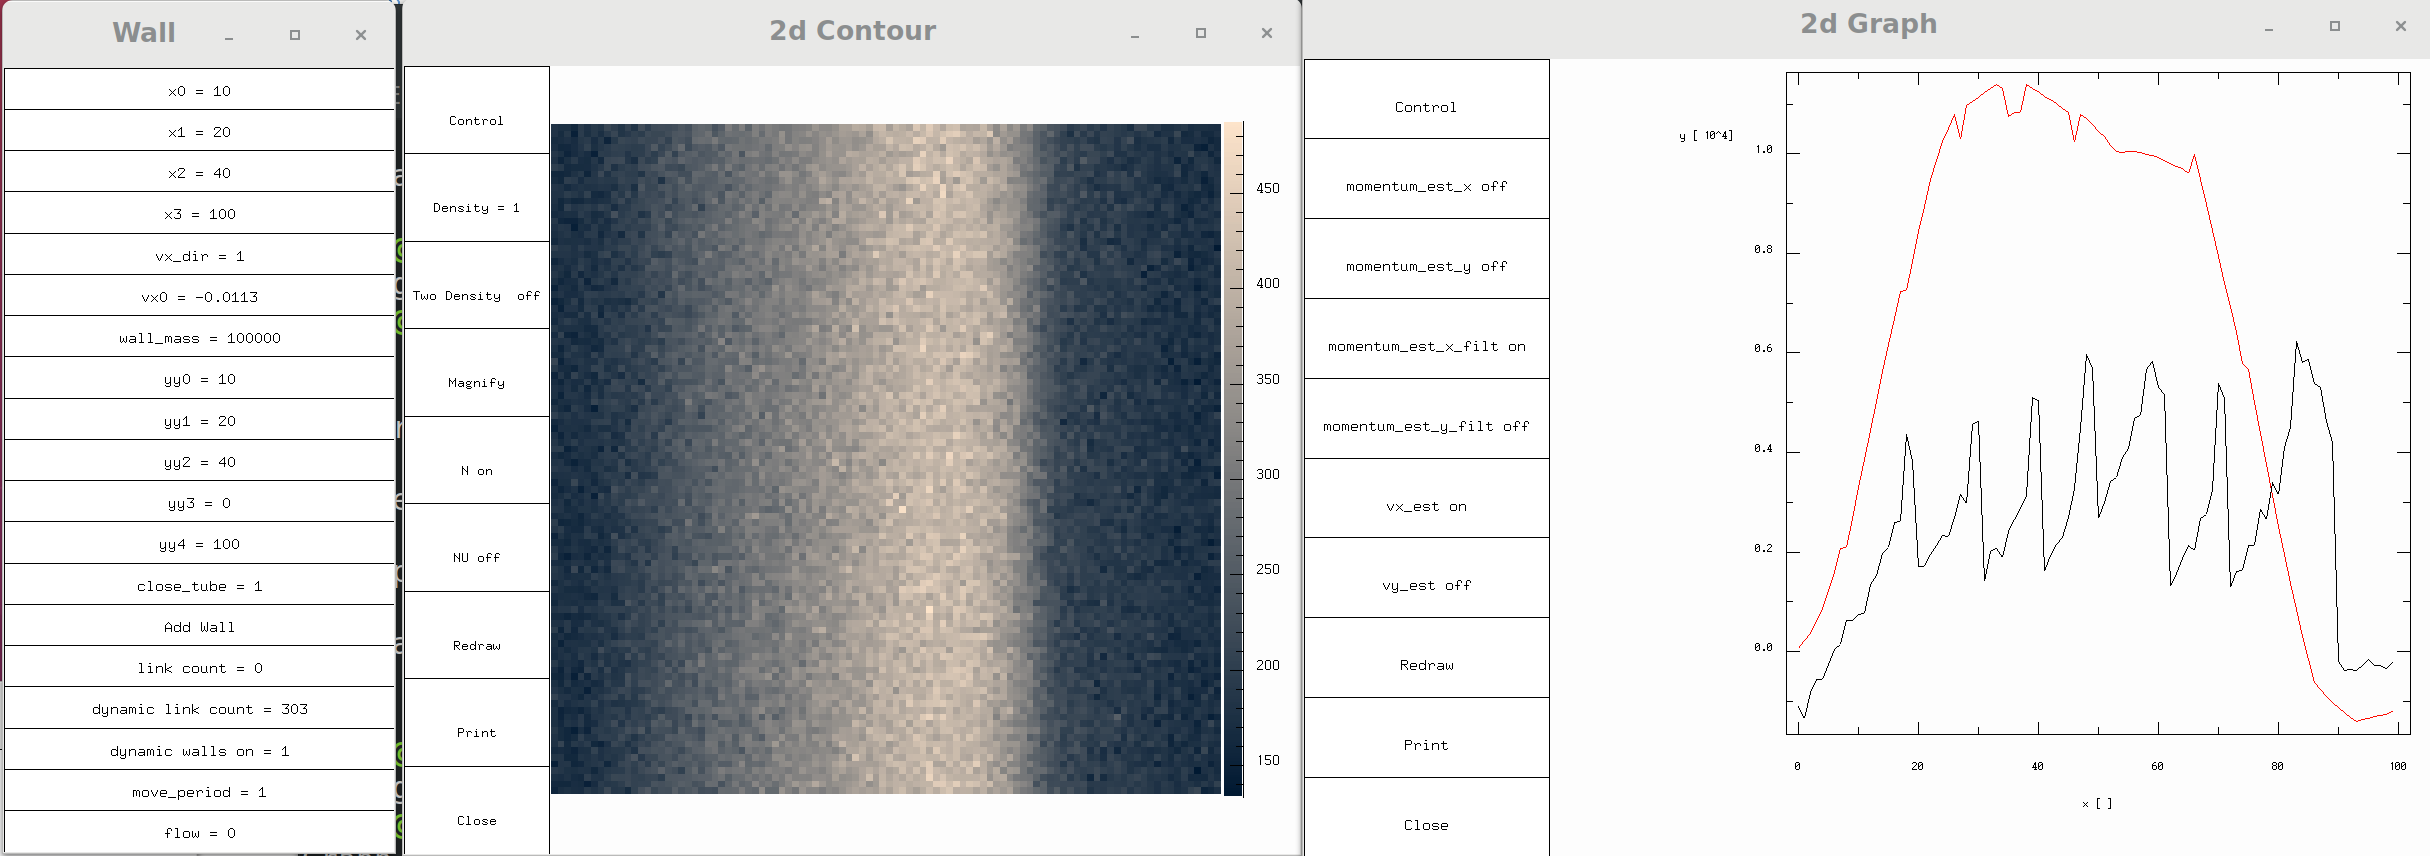
\includegraphics[scale=0.2]{ms2p1.png}
\caption{\label{fig} Several Iterations Later: the wall velocity begins to change and move towards the lower density side of the box. There seems to be some sloshing/ reflections of the particles as the velocity is now negative}
\end{figure} 

  
\end{itemize}
Some of these milestones have been revised based on information obtained while developing the code to run said simulations. 
\begin{itemize}
  
  \item Decrease the amount of particle leakage. Find a way to measure particle leakage.
  
  \item Create an architecture in the code to simplify the addition of multiple line shapes, the manipulation of their characteristics and states like mass, velocity, position. This architecture should also include the ability to create diagonal lines. (In Progress)
  
  \item develop code to allow for shapes to rotate about a center of mass or a fixed point.
  
 
Additional long term milestones could include the addition of rotating walls, hinges to connect walls, flexible walls. These features may be unrealistic with the available time, but could prove to be useful in creating more complex simulations.
\end{itemize}
\section{Timeline}
\begin{itemize}
  \item Tuesday, April 17th: Have milestone 1 and 2 completed - achieved except number 1
  \item Thursday, April 19th: Have milestone 3 started - achieved, but particles still leaking
  \item Tuesday, April 24th: Have milestone 3 completed and 4 started. (slightly behind, 3 is not entirely completed yet)
=======
The primary objective is to have a shape/line/wall that can move and appear to push lattice gas particles like a physical wall would do in the real world. These walls in the existing program can be easily moved, but as the wall moves it will move through some particles creating a leakage. To compensate for this leakage, particles are subtracted from the lattice sites on the leaving side of the wall and the same number are added to the arriving side of the wall. The sum of the particles added or removed must be zero, must not create negative particle densities. The number of particles added is taken randomly from a flat distribution. 
\section{Research Group}
David Jedynak programs 
\section{Completed Milestones}

\section{Future Milestones}
This project will depend on the a previously developed integer lattice gas simulation: "LG2d.c". This simulation already has features similar to the ones proposed in this project such as static walls that reflect particles. Code will be added to the LG2d.c simulation to observe how particles behave when the wall is dynamic instead of static walls. 
\begin{itemize}
  \item Simulate with stationary wall and particles initially moving uniformly perpendicular to the wall. Observe how the wall influences the particles' average velocity.  
  \item Develope code to simulate a moving wall(independent of particle collisions). Simulate with initailly stationary particles. Observe how the wall influences particles average velocity. Compare results to item 1 on this list. They should have a similar result because both particles and wall are both moving with the same velocity relative to eachother.
  \item Develope code to simulate a stationary tube. Place two dynamic walls on each end of the tube with particles inside this chamber. Move walls inward. Verify particles do not leak out. Observe how the particle density changes as the chamber decreases in size. Observe the forces on the walls as the chamber size changes.
  \item Develope code to make wall momentum to be dependent on particle collisions. Simulate a hollow, hoizontal, stationary tube with one horizontally movable, vertical wall. place gasses in each side of the vertical wall with different densities. Observe the movement of the movable wall. The wall should stop moving when both particle desities equalize.\newline
\vspace{5mm}\newline
Additional long term milestones could include the addition of rotating walls, hinges to connect walls, flexible walls. These features may be unrealistic with the avaliable time, but coule prove to be useful in creating more complex simulations.
\end{itemize}
\section{Timeline}
\begin{itemize}
  \item Tuesday, April 17th: Have milestone 1 and 2 completed
  \item Thursday, April 19th: Have milestone 3 started (even if leaking particles)
  \item Tuesday, April 24th: Have milestone 3 completed and 4 started. 
>>>>>>> 1e1b30a4df3ad27c758e98ed13c6c904fd4f09cb
  \item Thursday, April 26th: Have 4 completed.
  \item Tuesday, May 1st: Have 5 started/partially functional.
  \item Thursday, May 3rd: Have 5 completed.
  \item Tuesday, May 8th: Have results and project deliverables compiled and ready to turn in.
\end{itemize}
<<<<<<< HEAD
\end{document}
=======
\end{document}
>>>>>>> 1e1b30a4df3ad27c758e98ed13c6c904fd4f09cb
